\documentclass[journal,10pt,twocolumn]{article}
\usepackage{graphicx, float}
\usepackage[margin=0.5in]{geometry}
\usepackage{amsmath, bm}
\usepackage{array}
\usepackage{booktabs}
\usepackage{xfrac}
\usepackage[utf8]{inputenc}
\providecommand{\norm}[1]{\left\lVert#1\right\rVert}
\let\vec\mathbf
\newcommand{\myvec}[1]{\ensuremath{\begin{pmatrix}#1\end{pmatrix}}}
\newcommand{\mydet}[1]{\ensuremath{\begin{vmatrix}#1\end{vmatrix}}}

\title{\textbf{optimization Assignment}}
\author{Harsha sai sampath kumar}
\date{october 2022}

\begin{document}

\maketitle
\paragraph{\textit{\large Problem Statement} -The maximum volume of right circular cone having slant height 3m
 is}

\section*{\large Solution}

\begin{figure}[H]
\centering
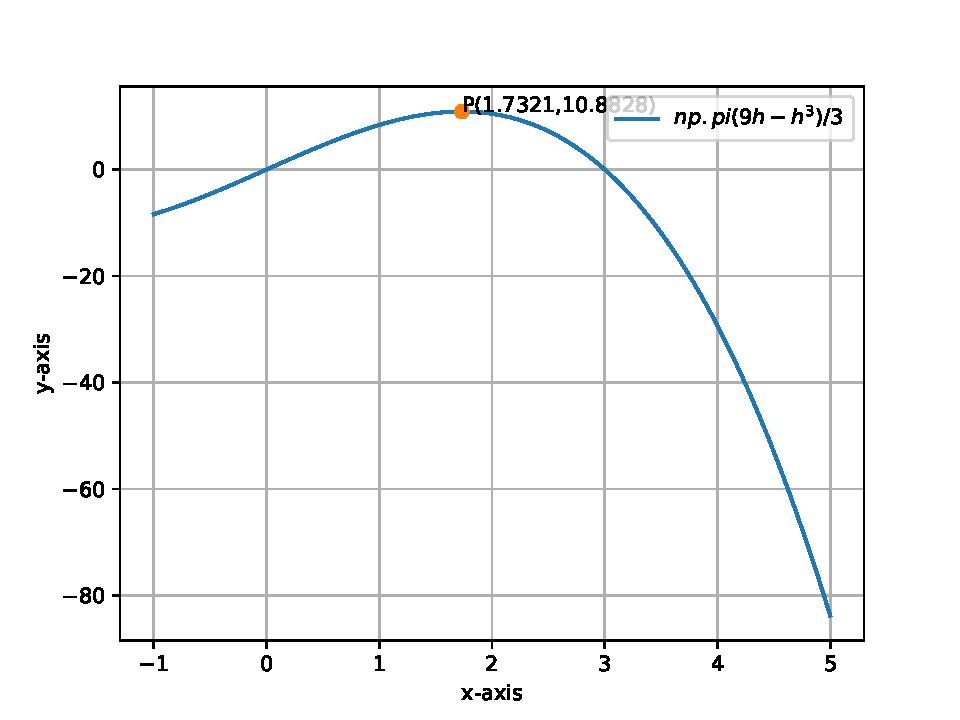
\includegraphics[width=1\columnwidth]{fig}
\caption{}
\end{figure}

   
  
   By Using Pythagoras theorem,we get
\begin{eqnarray}
h^2+r^2=3^2
\end{eqnarray}
\begin{eqnarray}
r^2=9-h^2
\end{eqnarray}
 volume of cone
\begin{eqnarray} 
V=\frac{1}{3}\pi r^2h
\end{eqnarray}
 Now,let us substitute above attained value of r in the  volume
\\
\begin{eqnarray}
V=\frac{1}{3}\pi( 9-h^2)h\\
\end{eqnarray}
\begin{eqnarray}
V=\frac{1}{3}\pi( 9h-h^3)
\end{eqnarray}

  


\section*{\large Gradient Ascent Method}

\begin{equation}
        x_{n+1} = x_n + \alpha \nabla f(x_n) \\
\end{equation}
\begin{equation}
        x_{n+1} = x_n + \alpha \nabla (\frac{(9x_n-x_n^3)\pi}{3}) \\
\end{equation}
 Taking $x_0 = 1, \alpha = 0.001$ and $precision = 0.00000001$, values obtained using python are:
\begin{align}
\boxed{\text{Maxima} = 10.88} \\
\boxed{\text{Maxima Point} = 1.732}
\end{align}
\end{document}
